\documentclass[paper=a4]{ctexart} % A4 paper and 11pt font size
\usepackage{fontspec,caption, xeCJK,amsmath,tocvsec2,extarrows, chngpage, adjustbox, clrscode}
\usepackage{listings}
\usepackage[T1]{fontenc} % Use 8-bit encoding that has 256 glyphs
\usepackage[english]{babel} % English language/hyphenation
\usepackage{amsmath,amsfonts,amsthm,amssymb, enumerate} % Math packages
\usepackage{framed,floatflt}   
\usepackage{graphics}
\usepackage{graphicx}
\usepackage{picins}
\usepackage{lipsum} % Used for inserting dummy 'Lorem ipsum' text into the template

\usepackage{sectsty} % Allows customizing section commands
% \allsectionsfont{\centering \normalfont\scshape} % Make all sections centered, the default font and small caps
\usepackage{wrapfig}
\usepackage{fancyhdr} % Custom headers and footers
\pagestyle{fancyplain} % Makes all pages in the document conform to the custom headers and footers
\fancyhead{} % No page header - if you want one, create it in the same way as the footers below
\fancyfoot[L]{} % Empty left footer
\fancyfoot[C]{} % Empty center footer
\fancyfoot[R]{\thepage} % Page numbering for right footer
\renewcommand{\headrulewidth}{0pt} % Remove header underlines
\renewcommand{\footrulewidth}{0pt} % Remove footer underlines
\setlength{\headheight}{13.6pt} % Customize the height of the header

\numberwithin{equation}{section} % Number equations within sections (i.e. 1.1, 1.2, 2.1, 2.2 instead of 1, 2, 3, 4)
\numberwithin{figure}{section} % Number figures within sections (i.e. 1.1, 1.2, 2.1, 2.2 instead of 1, 2, 3, 4)
\numberwithin{table}{section} % Number tables within sections (i.e. 1.1, 1.2, 2.1, 2.2 instead of 1, 2, 3, 4)

\lstset{
        keywordstyle=\color{blue}, %设置关键字颜色
        commentstyle=\color[cmyk]{1,0,1,0}, %设置注释颜色
        frame=single, %设置边框格式
        escapeinside=``, %逃逸字符(1左面的键),用于显示中文
        breaklines, %自动折行
        extendedchars=false, %解决代码跨页时,章节标题,页眉等汉字不显示的问题
        xleftmargin=2em,xrightmargin=2em, aboveskip=1em, %设置边距
        tabsize=4, %设置tab空格数
        showspaces=false %不显示空格
       }

\setlength\parindent{0pt} % Removes all indentation from paragraphs - comment this line for an assignment with lots of text

% ----------------------------------------------------------------------------------------
% TITLE SECTION
% ----------------------------------------------------------------------------------------
\newcommand{\horrule}[1]{\rule{\linewidth}{#1}} % Create horizontal rule command with 1 argument of height
\title{
  \normalfont \normalsize 
  \textsc{\\~\\~\\~\\~\\~\\University of Science and Technology of China} \\ [25pt] % Your university, school and/or department name(s)
  \horrule{0.5pt} \\[0.4cm] % Thin top horizontal rule
  \huge 基于Inferno的集群与并行计算框架 \\ % The assignment title
  \horrule{2pt} \\[0.5cm] % Thick bottom horizontal rule
}

\newcommand{\n}{\\\indent}
\author{\Large{阮震元~~~~解宇飞~~~~杨智~~~~刘旭彤}\footnote{阮震元~:~PB13011009,联系方式rzyrzyrzy2014@gmail.com,科技实验楼1406系统设计室}
\setcounter{footnote}{-1}
\footnote{解宇飞~:~PB13011001~~~~杨智~:~PB13011079~~~~刘旭彤~:~PB13011072}
} % Your name
\date{} % Today's date or a custom date

\usepackage{enumitem}

\lstset{
        language=text,
        keywordstyle=\color{blue}, %设置关键字颜色
        commentstyle=\color[cmyk]{1,0,1,0}, %设置注释颜色
        frame=single, %设置边框格式
        escapeinside=``, %逃逸字符(1左面的键),用于显示中文
        breaklines, %自动折行
        extendedchars=false, %解决代码跨页时,章节标题,页眉等汉字不显示的问题
        xleftmargin=2em,xrightmargin=2em, aboveskip=1em, %设置边距
        tabsize=4, %设置tab空格数
        showspaces=false %不显示空格
       }

\newcounter{newlist} %自定义新计数器
\newenvironment{denselist}[1][可改变的列表题目]{%%%%%定义新环境
\begin{list}{\textbf{\hei #1} \arabic{newlist}:} %%标签格式
{
\usecounter{newlist}
\setlength{\labelwidth}{22pt} %标签盒子宽度
\setlength{\labelsep}{0cm} %标签与列表文本距离
\setlength{\leftmargin}{0cm} %左右边界
\setlength{\rightmargin}{0cm}
\setlength{\parsep}{0ex} %段落间距
\setlength{\itemsep}{0ex} %标签间距
\setlength{\itemindent}{44pt} %标签缩进量
\setlength{\listparindent}{22pt} %段落缩进量
}}
{\end{list}}%%%%%      


\begin{document}

\maketitle % Print the title
 
% 目录
% 可以直接编辑toc文件来更改目录
\clearpage
\setcounter{section}{0}
\setcounter{subsection}{0}
\setcounter{subsubsection}{0}
\tableofcontents
\clearpage
% 改变层次目录来达到section和subsection默认不编号(需要tocvsec2包)

\section{可行性研究报告}

\subsection{理论依据与技术依据}

\subsubsection{Sytx协议及其具体实现}

Inferno的文件系统协议(或Sytx)是贝尔实验室九号项目所开发的针对于分布式操作系统的网络协议,作用是链接系统内的组件.Inferno系统中文件是核心,这些文件代表了视窗、网络连接、进程、以及其他存在于操作系统中的各种元素.不同于NFS,Styx的用途是把数据缓存起来,并提供虚拟文件的机制(例如/proc用以表示进程).\n
在Inferno系统中,Inferno服务器(Inferno server)是被用来被Inferno进程访问的并提供分等级文件系统(文件树)的代理.一个服务器响应客户端的请求并导引文件树中的具体位置,同事可以对文件进行创建、删除、读写等操作.\n
对于某个服务器来说,连接是通过一个客户端和服务器间的双向的通信通道来实现的.客户端可能是单一的,也可能有多个客户共享同一连接.一个服务器文件的文件树通过bind和mount命令联结到一个进程组的命名空间上.这样,组内进程就是服务器的客户端:对于文件的系统调用就被翻译为请求和响应,并得到相应的服务.\n 
      Inferno的文件协议,Sytx,就是用于处理客户端和服务器间的消息(message)的.目前我们组所用的Sytx版本是和9P2000一致的.客户端给服务器传递请求(T-messages).相应的,服务器返回响应给客户端(R-messages).这样就构成了基本的发送和接收机制.关于message的样式,这里就不再赘述.不过值得一提的是fid——一个客户端用来辨认服务器上当前文件的32位无符号整型.\n 
      Styx在客户端及服务器端提交如下的消息.这些消息对应到虚拟文件系统层的进入点,所有的服务器都必须实现这些消息:
\begin{enumerate}
\item version : 交涉协议的版本.
\item error : error.
\item flush : 终止消息.
\item auth, attach : 打开连接.
\item walk : 走访目录层次结构.
\item create, open : 准备一个用来写入/读取既有或新增文件的fid.
\item read, write : 发送数据给文件或从文件接收数据.
\item clunk : 抛弃fid.
\item remove : 从服务器移除文件.
\item stat, wstat : 查询或变更文件属性.
\end{enumerate}
这些具体实现中,有几个是我们工程的技术依据:
\begin{enumerate}
\item walk message : walk消息使得服务器变更当前的与fid相联系的文件为一个在目录中旧的“当前文件”或者某一个它的子目录.Walk返回一个新的fid,这个fid指向于该文件.通常,客户为根目录保留fid,然后通过walk从根fid进行导引.
\item attach,auth message : attach消息用来从客户端的用户向服务器提供一个连接点(introduction).这条消息识别用户并选择文件树去访问.attach消息会使客户端会拥有一个指向目标文件树根目录的连接,当然这个目录通过fid来被识别.Auth消息包含一个afid,用来进行认证.一旦认证协议完成,相同的afid会被attach提供给用户来保证成功进入并获取服务.
\item stat,wstat :stat消息获取文件信息.Stat字段包括文件名,读写、执行权限,访问和修改次数,所有者和组的信息.Wstat允许默写文件的属性被做某些改动.
\item flush : flush信息可以终止某个请求.当服务器收到 Tflush,它就不会回复带有oldtag标记的消息并立刻发送Rflush.客户端必须等待直到得到Rflush.这时oldtag会被回收.
\item write,read,open,create,remove功能都如上面简介介绍.
\end{enumerate}
~\n  另外,Styx对于安全性也做了一定工作,提供了许多安全机制来处理会影响系统整体性和安全性的危险动作.统一的文件通信协议包含着用户和组的识别码.比如,在收到一个打开文件请求时,服务器会检查并匹配用户id.这个机制和通用操作系统比较类似.Styx用通过网路连接的文件系统方式提供远程资源.这种获取远程资源的方式对应用程序是透明的,所以认证不需要特别提供.例如,在inferno中,客户端和服务器间的通信渠道中会包含许多加密和消息摘要的协议.与通用文件服务器和一些电话通讯领域一样,所有对于资源的运用都会经过一定的认证,这也保证了远程管理的安全性.\n
  值得一提的是Styx协议将请求翻译为必要的字序列并将其在通信通道中传递.所以Styx协议适应于ISO标准的OSI Session Layer Level.所以它独立于机器结构并成功地应用于不同指令集和数据格式的机器中.

\subsubsection{ns - 显示当前命名空间}
 在立项依据中,我们简要介绍了命名空间的概念,在Inferno系统中,命名空间是一系列挂载点(mount points)和绑定(binds)的集合,与UNIX系统的挂载点相似.在Inferno系统中,你可以把一个使用styx协议的服务器挂载在一个文件描述符上(如一个网络连接,或者一个程序的管道),因此,挂载在命名空间中引入了一个新的文件树;另一方面,挂载还可以仅仅使命名空间的一部分作为一个别名出现在另一个命名空间中.\n
命名空间包括两个部分:常规路径,以“/”开始;和一个“特殊”的路径集合,以“\#”开始,后面跟单个字符.这些特殊路径是内核设备,为内核服务的文件树,频繁访问的硬件(如硬盘)或者内核数据结构(如处理器).只有命名空间中的常规路径可以通过bind、mount、unmount指令修改.ns命令用来打印当前的命名空间,在shell中执行ns命令打印出的是shell的命名空间.为了举例说明,下面是在初始Inferno下运行ns的输出:

\lstinputlisting{result/ns} ~\n
 如上面的输出所示,大多数行在常规文件系统中bind一个内核设备,例如\#U(Inferno根目录的内容)在/,\#m(鼠标)在/dev上,\#I(网络栈)在/net上.-a和-b选项分别表示第一条路径的内容出现在原来第二路径的后面和前面(第二条将会包含第一条路径和它自己的集合).如果出现选项-c,目标路径将允许文件创建.上面出现的命名空间是被Inferno初始化代码安装的,作为一种引导系统的方式给出一个合理的默认命名空间.
\n
挂载在命名空间中引入了一个外部文件树,就像UNIX系统mount一样,文件树被文件描述符上使用styx协议访问.内核通过翻译open/read/write/stat/stc系统调用成styx信息来控制styx部分,然后在返回值中回复信息.mount系统调用要求文件描述符使用styx协议通信.mount程序挂载3种类型的styx服务器拥有很方便的语法:

\begin{itemize}
\item mount /path/to/styx/file target, 通过打开/path/to/styx/file取得文件描述符
\item mount net!www.example.org!styx target, 通过访问net!www.a.org!styx取得文件描述符
\item mount {program} target, 开始程序并且用它的标准输入作为文件描述符
\end{itemize}

ns显示给定pid或者默认它本身的命名空间结构,以/prog/pid/ns的内容为基础,打印一系列bind和mount命令,如果它被执行,会重建一个相同的命名空间.如果任何涉及到的文件因mount或bind命令被改名,那么就显示文件的原始名字.

\subsubsection{bind, mount, unmount - 修改命名空间}

  bind和mount命令修改当前进程和在一个命名空间组中其他进程的命名空间,目标是一个存在的文件或当前将要修改的命名空间的目录名.对于bind,目标是一个已经存在的文件或当前命名空间下的目录名.在bind命令成功执行之后,目标文件名就是原来的东西起的一个别名;如果修改没有隐藏它,目标将依然指向他的原来的文件.源和目标必须是同一个类型,要么都是目录,要么都是文件.对于mount,源可以是一个shell命令,一个网址,或者一个文件名,如果源被花括号扩起来,那么它将作为一个sh命令的调用,如果源中包含感叹号或者没有文件,他将被作为一个网址.
\n
 bind和mount命令的工作可以被unmount命令撤消,如果给unmount两个参数,他会撤消相同参数的bind或mount命令,如果只给它一个参数目标上所有bind过和mount过的东西都会被撤消.注意,当使用bind或unmount命令时,内核设备名称中的\#字符必须被引号引起来否则shell会把它看做注释的开头. \n
修改命名空间的常用选项:
\begin{itemize}
\item  -b : mount和bind均有效.把源目录加入被目标目录代表的联合目录开头.
\item  -a : mount和bind均有效.把源目录加入被目标目录代表的联合目录结尾.
\item  -c : 这个选项可以加在上面两个选项上,用来允许在联合目录中的创建.当在联合目录中创建一个新的文件时,它将被放在联合目录中第一个mount或bind带有-c选项的元素中,如果那个目录没有写权限,将会创建失败.
\item  -q : 如果bind或mount失败,不打印诊断信息,安静退出.
\item  -A : 只对mount有效.在执行mount之前不认证服务连接.
\end{itemize}

\subsubsection{os - 寄主操作系统接口(对寄生安装的Inferno有效)}
os指令将使得我们使用C语言开发的程序在Inferno系统中运行.\n
  os使用使用cmd设备在寄主系统执行命令,如果存在-m选项,os会使用在挂载点的设备,否则将会被假设在/cmd下,如果必要还会被bind在本地命名空间下.-d选项将会导致命令运行在dir目录下,如果dir目录不存在或者无法访问就会报错,且指令不会执行.命令的标准输出和标准错误会出现在os命令本身的标准输出和标准错误上,os复制标准输入到远程命令的标准输入;如果命令没输入,就会重定向os的输入到/dev/null.当cmd终止后,os命令就终止了,它的退出状态返回的是cmd的退出状态.如果命令被杀死或退出(比如缺少输入或输出),寄主自己的进程控制办法将试图杀死仍在运行的cmd,-b(background)选项将制止这个行为.-n选项导致cmd在低于正常优先级下运行.-N选项把低优先级设置为特殊的等级,从1到3.

\subsubsection{cpu - 执行一个远程的命令}
cpu命令向主机拨号(使用tcp网络如果网络没有显式给出).连接后,向外传输本地的命名空间并执行远程机器上的指令.本地命名空间对于/n/client中的命令是可见的;本地的设备文件被bind到了远程设备目录下.如果命令没有给出,那么/dis/sh就处在运行之中. \n
-C选项设定了authentication被摘要或者加密的算法,具体的摘要算法有:MD4,MD5等,具体的加密算法有:RC4,DES,CBC,ECB等算法.默认的是不用任何算法.

\subsubsection{通信模式 - 主从模式}
之前我们调研了其他并行框架如MPI, CUDA, OpenMP等背景与实现方式.纵观MPI,它的通信模式主要有4种: 
\begin{itemize}
\item 标准通信模式:对等模式与主从模式.
\item 缓存通信模式
\item 同步通信模式
\item 就绪通信模式
\end{itemize}
~\n
经过深入了解,我们决定模仿MPI的主从模式去实现我们的并行计算框架.因为基于Inferno强大的分布式特点,我们可以简单的用bind的命令将远程的Inferno节点的资源挂载在本地,亦或是用cpu命令直接在远程端运行给定程序.所以我们可以选择一台节点当主节点,然后将其余从节点全部挂载在主节点上.由主节点分发任务,响应从节点请求,进行从节点间调度等等.\n
\begin{figure}[htbp]
  \centering
  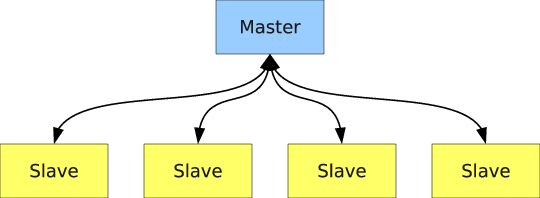
\includegraphics[width=4.8in,height=1.5in]{pic/master-slave.png}
  \caption{主从模式}
\end{figure}
基于主从模式的通讯方式在Inferno下开发并行框架可以大大加快我们推进速度.

\subsubsection{file2chan - 节点间通讯}
因为我们要实现并行计算框架,一个亟待解决的问题就是如何做节点间通讯.最初我们的想法是直接用一个文件来做共享池.然而后来在此基础上进行实现时发现困难重重:
\begin{enumerate}
\item 直接用文件做共享难以解决同步的问题.因为直接用文件做共享池,这样在运行时没法动态的加锁,解锁,不方便解决同步问题.
\item 难以实现主节点的动态任务分配.
\item 难以实现主节点对从节点请求的动态响应.
\item 光是一个文件难以做到传输各种格式不同的通讯信息.
\item 直接在磁盘中暴露中间计算内容,缺少加密.
\end{enumerate}
~\n
经过我们重重调研,发现Inferno提供了一个叫做file2chan的脚本工具.\n
file2chan是一个sh的可加载模块,可以在命名空间中创建一个可以由shell脚本决定其性质的文件.file2chan在命名空间中创建一个文件名,同时产生一个新的线程来为这个文件服务,如果成功了,环境变量\$apid就会被设置成新线程的pid,否则返回一个错误状态(non-nil).readcmd、writecmd和closecmd都应该是可执行的指令块.之后,每当一个进程从文件名读入,就会调用readcmd;每当一个进程对文件名写入,就会调用writecmd;每当一个从文件名打开的文件关闭,就会调用closecmd.\n
如果我们采用file2chan,则可以轻松的解决上述问题.具体设想与实现可以参考概要设计报告部分.

\subsection{创新点}

\subsubsection{实现MapReduce计算模型}
尚未有人、或极少人在Inferno上做过并行计算.然而,Inferno系统本身的特性使得它能很方便的实现并行计算.为了进一步完善我们小组的并行计算模型,我们也在Inferno上实现了MapReduce这一编程模型.通过MapReduce, 我们可以把一个大作业拆分成多个小作业,而用户只需要决定拆分成多少份,以及定义作业本身.因此,不熟悉并行编程的程序员也能充分发挥分布式系统的威力.事实证明,Inferno在实现并行计算框架这一点上较其它系统有天然的优势,只要进行少量的工作就完成了MapReduce在Inferno上的移植.

\subsubsection{多节点视为整体的一个节点}
集群是一组相互独立的、通过高速网络互联的计算机,它们构成了一个组,并以单一系统的模式加以管理.如今主流的集群实现方式中,集群中节点间的数据交换通过数据共享空间或者点对点的通信实现,各个节点事实上并不能真正成为一个整体,例如基于MPI(Message Passing Interface)的并行框架.而inferno通过导入Namespace(命名空间),使所有的资源都以分层次的文件的形式存在于文件系统中,因此应用程序可以以同样的方式访问远程的节点和本地节点.故而虽然这个系统上包含了很多的节点, 但是在用户和应用程序看来, 这就像是一个节点一样. 

\subsubsection{Inferno在64位平台上的移植}
最新的inferno第四版发行于2004年,支持的平台有ARM,PA-RISC,MIPS,PowerOC,SPARC,X86.但如今市面上的平台基本上都是64位的了,因此要想在64位的平台上运行inferno,就要进行移植.为了让Inferno能成功地在市面上绝大多数电脑上运行,把更多的平台纳入我们的并行框架中,我们修改了Inferno的部分代码,将其移植到了64位的平台上.

\subsubsection{以外部解释器的形式实现并行计算}
之前调研了其他著名并行计算框架的使用方式:
\begin{itemize}
\item CUDA, MPI : 用户根据具体的MPI实现框架(Intel MPI, OpenMPI等)给定的API接口,调用具体的库函数,进行串行代码的并行化移植.
\item OpenMP : 在要并行的代码块前加预处理指令\#pragma.编译器编译时则自动会链接OpenMP库,编译出并行化代码.
\end{itemize} 
~\n
我们借鉴了OpenMP的并行化的技术,提出了使用外部解释器思想.我们是针对Inferno的shell实现并行计算框架,而shell并不需要编译,是通过Inferno中自带的sh逐行解释执行的.然而直接对Inferno中的sh动手脚是不可能的,sh部分代码量高达好几万行,没有注释并且还使用了部分内核接口.我们之前调研发现Inferno的shell本身就自带bind, cpu, file2chan等工具,可以直接编写能在Inferno的shell上运行的并行化代码.所以我们决定实现一个外部解释器,将用户的串行代码按照给定的需求解释成能直接在Inferno的shell中直接运行的并行化代码.\n

这点和OpenMP又有极大的不同,OpenMP并行化的程序在运行时还需要调用OpenMP库.而我们则要实现串行代码再经过解释器解释之后可以直接在Inferno的sh上运行,不需要再调用其他库,可以说是得到了在Inferno平台下“完全并行化”的代码.

\subsubsection{以C语言而非Limbo语言来编写解释器程序}
在Inferno里,我们需要用Limbo来写应用程序.Limbo是一种用于分布式系统的编程语言.然而Limbo是一门不流行的语言,相关文档较少,因此学习这门语言势必需要花费较多的时间与精力.但是,假如我们是以应用程序的形式在别的系统上运行Inferno,那么我们就可以通过os这条命令,来间接地在Inferno上运行host机器上的程序.于是,我们小组选择了用C语言来写解释器,通过os命令来间接地让解释器在Inferno上运行,大大加快了开发进度.

\subsubsection{对file2chan的读写方法封装,实现一个文件完成各种类型通讯}
此部分具体见概要设计报告中的sharedPool - 节点间通讯一节. 
\subsection{概要设计报告}

\subsubsection{总体路线}
在理论依据部分和创新点部分已经提及了我们的部分设计思路.我们的最终目的就是实现一个外部解释器,可以根据需求将用户给定的串行程序翻译成基于主从模式的,可以在Inferno的shell环境下直接运行的并行化代码. \n
总的开发阶段可以划分为如下两个部分:
\begin{itemize}
\item 自己先摸索出在Inferno中将串行程序并行化改写的方法,并对具体语句总结出一套模式化改写规则(如对一段for改如何改写)
\item 开发解释器,按照之前总结的改写规则将串行代码翻译为并行代码.
\end{itemize}
~\n
对于第一个阶段我们已经完成部分,具体成果如下所示.

\subsubsection{一个串行程序}
\lstinputlisting{code/workerSerial.sh}
~\n
先简要的解释一下这个程序.subfn fac实现了一个计算阶乘的子函数.subfn c实现了一个组合数的子函数.subfn calc实现了一个统计函数,对于给定的n可以统计有多少个$r\leq n$满足$C(n,r) > 1000000$.\n
最外层则是一个i从23到100变化的for循环,将所有的calc(i)相加输出.值得注意的是在Inferno下任何算数运算都采用后缀表达式并通过调用内嵌子函数expr完成.\n
本身这个程序没有任何意义,举这个程序为例子只是为了演示如何将一段串行代码并行化.

\subsubsection{改写的主从式并行代码}
\paragraph{master部分}
\lstinputlisting{code/master.sh}
\paragraph{worker部分}
\lstinputlisting{code/worker.sh}  

\subsubsection{sharedPool - 节点间通讯}

首先在master部分我们通过file2chan定义了一个虚拟文件/tmp/sharedPool用作节点间通讯.然而由于节点间通讯消息种类十分繁杂(例如主节点给从节点分配任务,从节点计算完毕将结果提交给主节点),各自的格式也都不一样.如果开多个file2chan则必定会带来管理的紊乱.于是我们创新性的采用封装了file2chan的read,write方法使得一个file2chan可以完成各种类型的信息通讯. \n
当想使用sharedPool进行消息通讯时,首先向sharedPool写入具体的操作类型.sharedPool中的我写好的read的方法会读取给定的操作类型,并在内部根据给定操作类型切换响应的模式来应对. \n
例如在我这个例子中,当worker想要向master索求数据时先向sharedPool写入get,然后再对sharedPool执行读取操作即可读到主节点分配给它数据.当worker计算完成,要把结果反馈给master时就先向sharedPool写入put,然后再往sharedPool写入算得的数据,此时就会触发sharedPool的write方法,自动将本次worker向master提交的结果计入总结果.

\subsubsection{节点间通讯同步}
Inferno本身已经对file2chan做了同步处理,当你往里写时就不能读,读时就不能写.一个节点在读的同时其他节点就不能读,一个节点在写时其他节点就不能写.我们唯一要做的是保持事务的原子性.因为我们之前封装了file2chan的read,write方法使得其支持各种类型的通讯信息,这带来方便也带来了弊端.例如一个节点往sharedPool中写入了get,于是sharedPool内部切换为get模式等待这个节点来取数据.然而若在此时另外一个节点计算完了数据想向sharedPool提交数据,于是在之前那个节点读数据之前又往sharedPool写入了put,使得其内部转换为了put模式.那么之前那个节点再读数据就会发生错误.我们要做的就是使得一个节点向sharedPool指明操作类型之后的下一步只接受这个节点的请求(即事务的原子性). \n
我们的实现方法是当sharedPool接收到a节点指定的命令类型之后,马上锁定a节点.下一步只接受来自a节点的请求.如果b节点此时再往sharedPool写入就会无效.然而这还有一问题就是要让b节点等待一会再执行写入操作,而不是直接跳过这次写入操作,否则会导致信息丢失.如果file2chan可以提供write方法的返回值,通过告诉节点b执行write方法的成功与否来让他继续执行或等待.\n
可惜的是Inferno中没有提供对file2chan中read,write方法返回值的支持.于是我们创新性的采用文件名的方式来解决这个问题.由于每个节点都对应一个进程号pid,当pid为x的节点写操作成功时就在/tmp目录下生成一个名为x的文件.当pid为x的进程检测到目录中有x这个文件时就知道了它本次write操作是成功的,可以删掉这个文件(消除痕迹)继续往下执行,否则等待.通过方式我们绕开了Inferno中file2chan的限制,成功的实现了同步效果.

\subsubsection{执行效果}
为了便于调试,我们将master和worker的屏幕输出信息都重定向到了日志文件.执行环境是我和刘旭彤的电脑(通过wifi连接在同个局域网下),我的机子充当主节点,刘旭彤的机子充当从节点.在我的Inferno中执行cpu master.sh 192.168.1.1(局域网中我的IP) 192.168.1.10(局域网中刘旭彤的IP)便可实现两个节点对跑. \n
运行完毕后/pool目录中有3个日志文件.\n
\paragraph{liuxt-MacBookAir-Invalid-entry-length-DMI-table-is-broken-Stop.log}
\lstinputlisting{log/liuxt-MacBookAir-Invalid-entry-length-DMI-table-is-broken-Stop.log}
\paragraph{macbook.log} 
\lstinputlisting{log/macbook.log}
\paragraph{master.log}
\lstinputlisting{log/master.log}
~\n 可以看到我的机子(macbook,pid77)和刘旭彤的机子(liuxt-MacBookAir,pid893)并行的完成了整个任务的计算. \n
同时我还比较了串行程序运行时间与两个节点并行化运行时间.对于这个例子,串行时间为1分32秒,两个节点并行化运行时间为56秒,可以看到加速比为1.6(小于2是因为节点间负载均衡问题以及节点间通讯调度时间)效果明显!

\subsubsection{Future Work}
由于任务调度是直接基于抢占式的,由于网络关系(我在这个例子中既充当了主节点又充当了从节点,作为从节点向主节点抢占任务的速度肯定快于刘旭彤)可以看到节点间负载并不均衡.所以我们下一步要做的首要工作是进行节点间负载均衡.\n
其次我们将继续摸索串行程序并行化的改写方法.当积累到一定程度时,并可开始解释器的编写工作.
\end{document}

%%% Local Variables:
%%% mode: latex
%%% TeX-master: t
%%% End: 





